\documentclass{article}

\usepackage{enumerate}

\usepackage{amsmath}

\usepackage{amssymb}

\usepackage{graphicx}

\usepackage{subfigure}

\usepackage{geometry}

\usepackage{color}

\usepackage{bm}

\usepackage{indentfirst}

\usepackage{array}

\usepackage{multirow}
\usepackage{float}
\usepackage{diagbox}
\begin{document}
\hrulefill
\thispagestyle{empty}



\begin{center}

\begin{large}

\sc{UM--SJTU Joint Institute \vspace{0.3em} \\ Physics Laboratory \\(VE215)}

\end{large}



\hrulefill



\vspace*{5cm}

\begin{Large}

\sc{{Laboratory Report}}

\end{Large}



\vspace{2em}



\begin{large}

\sc{{Exercise 3

\vspace{0.5em}



Transient Lab

}}

\end{large}

\end{center}





\vfill



\begin{table}[h!]

\flushleft

\begin{tabular}{lll}

Name: Xu Yiyang \hspace*{2em}&

ID: 518370910020\hspace*{2em}\\





\\



Date: 30 Oct 2019 



\end{tabular}

\end{table}



\newpage





\section{Goal}

\begin{enumerate}

\item

Apply the theory you learned on the step responses in 
rst- and second- order circuits to series RC and RLC circuits, which you will build in the lab.

\item
Build a series RC circuit, observe its responses to input square wave signal of varied frequency, and explain them based on the theory you learned:

\begin{enumerate}[$\bullet$]

\item

Relate the observed capacitor voltage and resistor voltage as functions of time to your pre-lab calculations

\item

Explain the changes of both output waveforms in response to the increase of the frequency of the input square wave signal

\item

Explain the amplitudes of the capacitor voltage and the resistor voltage related to the amplitude of the input square wave

\end{enumerate}

\item

Build a series RLC circuit, observe the three types of its responses to input square wave signal, and relate them to the theory you have learned. For the under-damped/ over-damped/ critical damped response, compare the resistance in the circuit measured in the lab with the critical resistance you calculated in the pre-lab.

\item

Build the simplest second-order circuit, an LC tank, and observe oscillations.

\end{enumerate}


\section{Introduction}

\subsection{First-order circuits}

Theoretically, the transient responses in electric circuits are described by differential equations. The circuits, whose responses obey the first-order differential equation

$$\frac{dx(t)}{dt}+\frac{1}{\tau}\cdot x(t)=f(t)$$

are called first-order circuits. Their responses are always monotonic and appear in the form of exponential function

$$x(t)=K_1\cdot e^{-\frac{t}{\tau}}+K_2$$

A first-order circuit includes the effective resistance R and one energy-storage element, an inductor L or a capacitor C.
In an RC circuit, the time constant is

$$\tau=RC$$

In an LC circuit, the time constant is

$$\tau=\frac{L}{R}$$

The fall time of a signal is defined as the interval between the moment when the signal reaches its 90\% and the moment when the signal reaches its 10\% level. Note that the 10\% level is reached between 2$\tau$ and 3$\tau$ . Approximately, you can assume falltime $\approx2.2\tau$ . After $t = 5\tau$ , the exponent practically equals zero.



\subsection{Second-order circuits}

Many circuits involve two energy-storing elements, both an inductor L and a capacitor C. Such circuits require a second-order differential equation description

$$\frac{d^2x(t)}{dt^2}+2\cdot\alpha\cdot\frac{dx(t)}{dt}+\omega_0^2\cdot x(t)=f(t)$$

thus they are called second-order circuits.

We will consider only second-order circuits with one inductor and one capacitor. The differential equation includes two parameters: the damping factor $\alpha$ and the undamped frequency $\omega_0$ which are determined by the circuit and its components.

For example, in the series RLC circuit, which you will build and study in this lab,

$$\alpha=\frac{R}{2\cdot L},\rm{and}\ \omega_0=\frac{1}{\sqrt{L\cdot C}}$$

while in the parallel RLC circuit,

$$\alpha=\frac{1}{2\cdot R\cdot C},\rm{and}\ \omega_0=\frac{1}{\sqrt{L\cdot C}}$$

Depending on the two parameters $\alpha$ and $\omega_0$, second-order circuits can exhibit three types of responses.

\subsubsection{The underdamped response}

If $\alpha<\omega_0$

$$x(t)=e^{-\alpha t}(K_1\cos(\omega t)+K_2\sin(\omega t))$$

where $\omega=\sqrt{\omega_0^2-\alpha^2}$

The underdamped circuit response involves decaying oscillations, which may last for many periods or for less than one period, depending on the damping ratio $\delta=\frac{\alpha}{\omega_0}$, which for the series RLC circuit 

$\delta=\frac{R}{2L}\sqrt{LC}=\frac{R}{2}\cdot\sqrt{\frac{C}{L}}$. Varying the values of R, L, C, affects the damping ratio $\delta$.

\subsubsection{The critically damped response}

If $\alpha=\omega_0$

$$x(t)=e^{-\alpha t}(K_1+K_2t)$$

and the circuit has the critically damped response.\newline

\indent The critically damped response does not involve oscillations.
\indent For the series RLC circuits, $\alpha=\omega_0$ corresponds to $\frac{R}{2L}=\frac{1}{\sqrt{LC}}$ or $R=R_{critical}=2\sqrt{\frac{L}{C}}$

If $L = 1mH$ and $C = 10nF$, then $R_{critical} \approx 632 \Omega$.

\subsubsection{The overdamped response}
If $\alpha>\omega_0$

$$x(t)=K_1\cdot e^{s_1t}+K_2\cdot e^{s_2t}$$

where $s_1=-\alpha+\sqrt{\alpha^2-\omega_0^2}$ and $s_2=-\alpha-\sqrt{\alpha^2-\omega_0^2}$

In the series RLC circuits, the overdamped solution is obtained if the resistance is larger that the critical resistance, such that $R>R_{critical}=2\sqrt{\frac{L}{C}}$

Notice that the larger resistance corresponds to the longer delay, and even the faster decay has a much longer fall time than the critically damped response. 
One of the most interesting features of series RLC circuits is that increasing the resistance above the critical value results in much longer fall time, or longer delays of responses in digital circuits. Among all monotonic responses, the critically damped is the fastest.

\section{Results and Discussion}

\subsection{First-order circuits}

\begin{table}[!h]

\begin{center}

\begin{tabular}{|c|c|c|}

\hline

The setting of the potentiometer  & Fastest circuit response & Slowest circuit response \\

\hline

$V_{ppk}$ input [V]		&	1.00	&	1.00	\\

\hline

$V_{ppk}$ output [V]	&	1.04	&	1.02	\\

\hline

Period $T$ of the input [ms]	&	10.000	&	10.000	\\

\hline

Rise Time of the Output [ms]	&	1.600	&	19.000	\\

\hline

Fall Time of the Output [ms]	&	1.900	&	18.000	\\

\hline

\end{tabular}
\caption{First-order circuits.}
\label{tab-1}
\end{center}
\end{table}
%---------------------------------
  \begin{figure}[H]
  \centering
  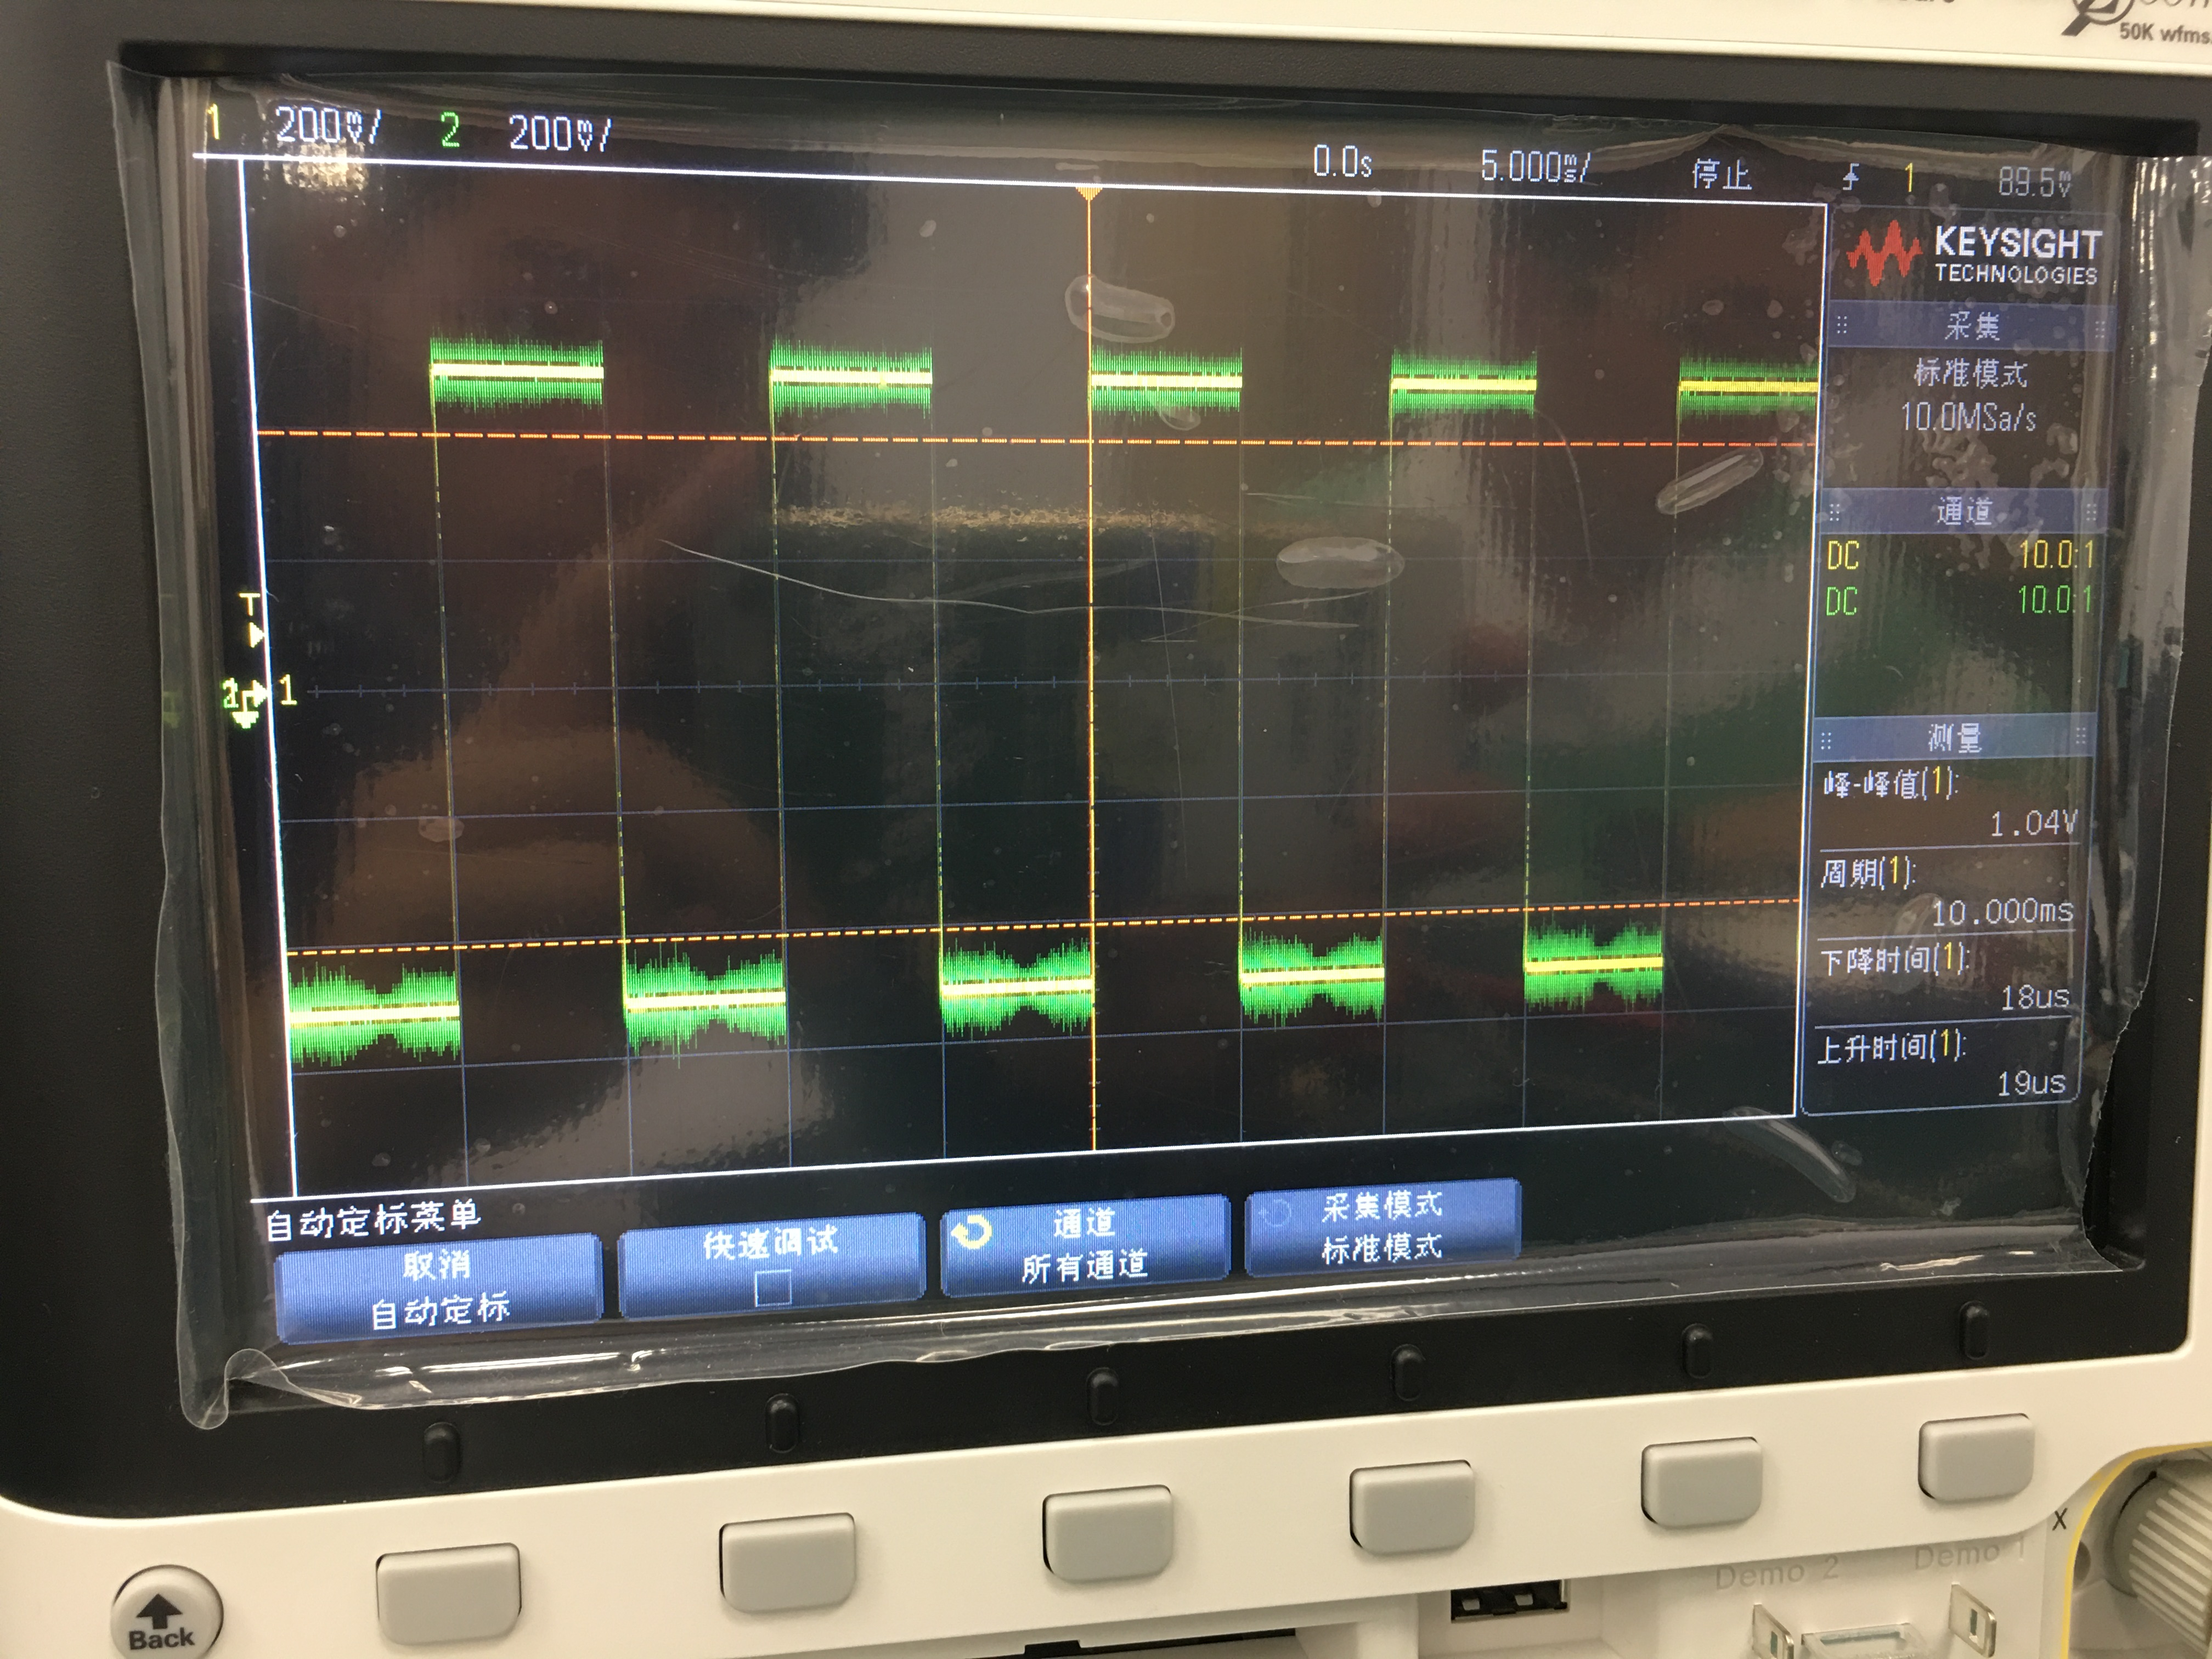
\includegraphics[width=.6\textwidth]{Figure2.jpg}
  \caption{fastest circuit response}
  \label{img} 
\end{figure}
%--------------------------------- 

%---------------------------------
  \begin{figure}[htp]
  \centering
  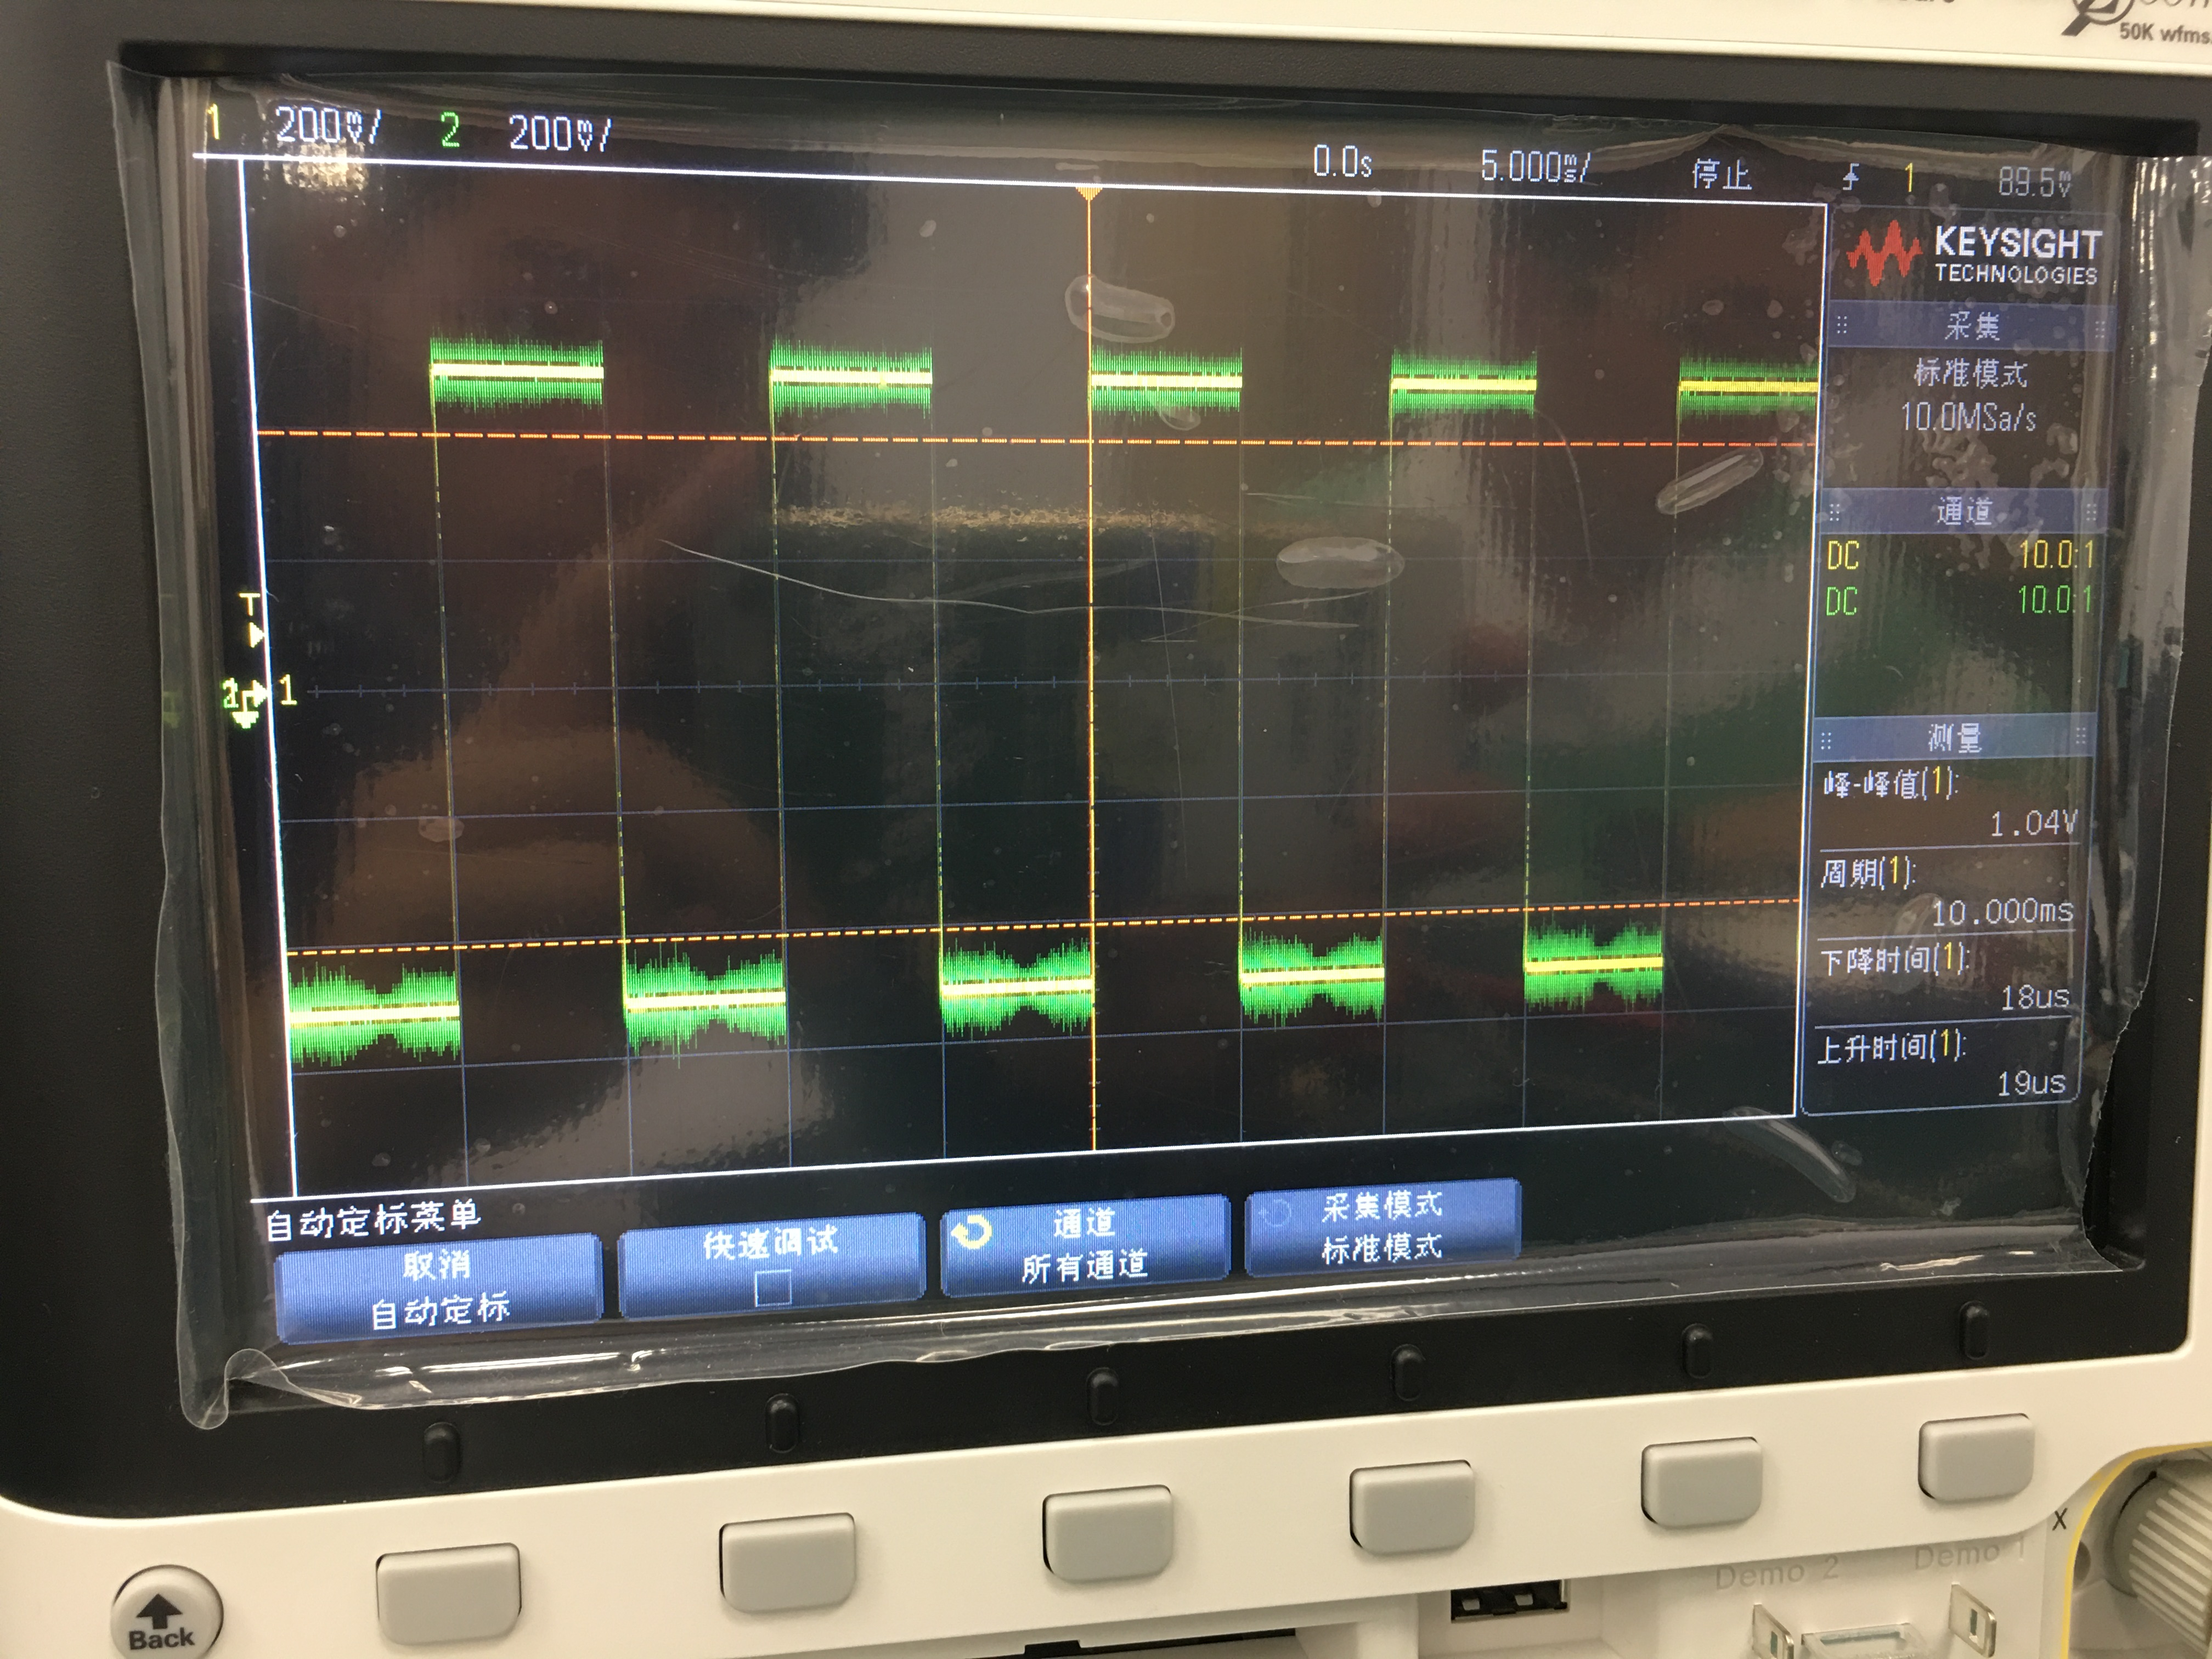
\includegraphics[width=.6\textwidth]{Figure2.jpg}
  \caption{Slowest circuit response}
  \label{img} 
\end{figure}
%--------------------------------- 

According to the table we obtained, the $\tau $ for the fastest circuit reponse is:
$$\tau=\frac{1.6+1.9}{2}\cdot\frac{1}{2.2}=0.795\,\rm{ms}$$

Theoretically,

$$\tau=RC=1000* 0.1\times 10^{(-6)}= 0.100\,\rm{ms}$$

Therefore, the relative error is $$error = \frac{0.795-0.100}{0.100}\times 100\% = 69.5 \%$$\\ This error is so huge and the reason will be discussed later in the discussion part.

Similarly, for the slowest circuit response,

$$\tau=\frac{19.000+18.000}{2}\cdot\frac{1}{2.2}=8.409\,\rm{ms}$$

Theoretically,
$$\tau=RC=11k \times 0.1\times 10^{(-6)}= 1.100\,\rm{ms}$$

Therefore, the relative error is $$error = \frac{8.409-1.100}{1.100}\times 100\% = 66.45 \%$$\\
Again, this error is huge. However, the magnitude of the error is close to the error presents in the fastest circuit response, so that we think there's some common error in these cases.

We can find that in both cases, the relative errors are not small enough to draw a correct conclusion. The possible error is because of the wrong value of resistance and the system error of the oscilloscope itself. 


\subsection{Second-order circuits}

\begin{table}[htp]

\begin{center}

\begin{tabular}{|c|c|c|c|c|}

\hline

& Resistance $R_p$ [$k\Omega$] & Rise Time [$ms$] & Fall Time [$ms$] & Time interval $\Delta t$ [$\mu s$] \\

\hline

\multirow{2}{*}{Under-damped}		&	0.481	&	$1.056\times 10^{-3}$	&	$1.060\times 10^{-3}$	&	3[$\mu s$]	\\

\cline{2-5}

&	134	&	$9.920\times 10^{-4}$	&	$9.320\times 10^{-4}$	&	2.6	\\

\hline

Critically damped	&	1.718	&	$2.028\times 10^{-3}$	&	$2.064\times 10^{-3}$	&	\multirow{3}{*}{\diagbox[height=3.5em,width=11em,dir=SE]{}{}}\\

\cline{1-4}

\multirow{2}{*}{Over-damped}	&	9.800	&	$1.602\times 10^{-2}$	&	$1.576\times 10^{-2}$	&	\\

\cline{2-4}

&	4.700	&	$7.86\times 10^{-3}$	&	$7.80\times 10^{-3}$	&	\\

\hline

\end{tabular}

\caption{Second-order circuits.}

\label{tab-2}

\end{center}

\end{table}

First, we consider the under-damped situation. The following figure shows the experimental situation.

%---------------------------------
  \begin{figure}[H]
  \centering
  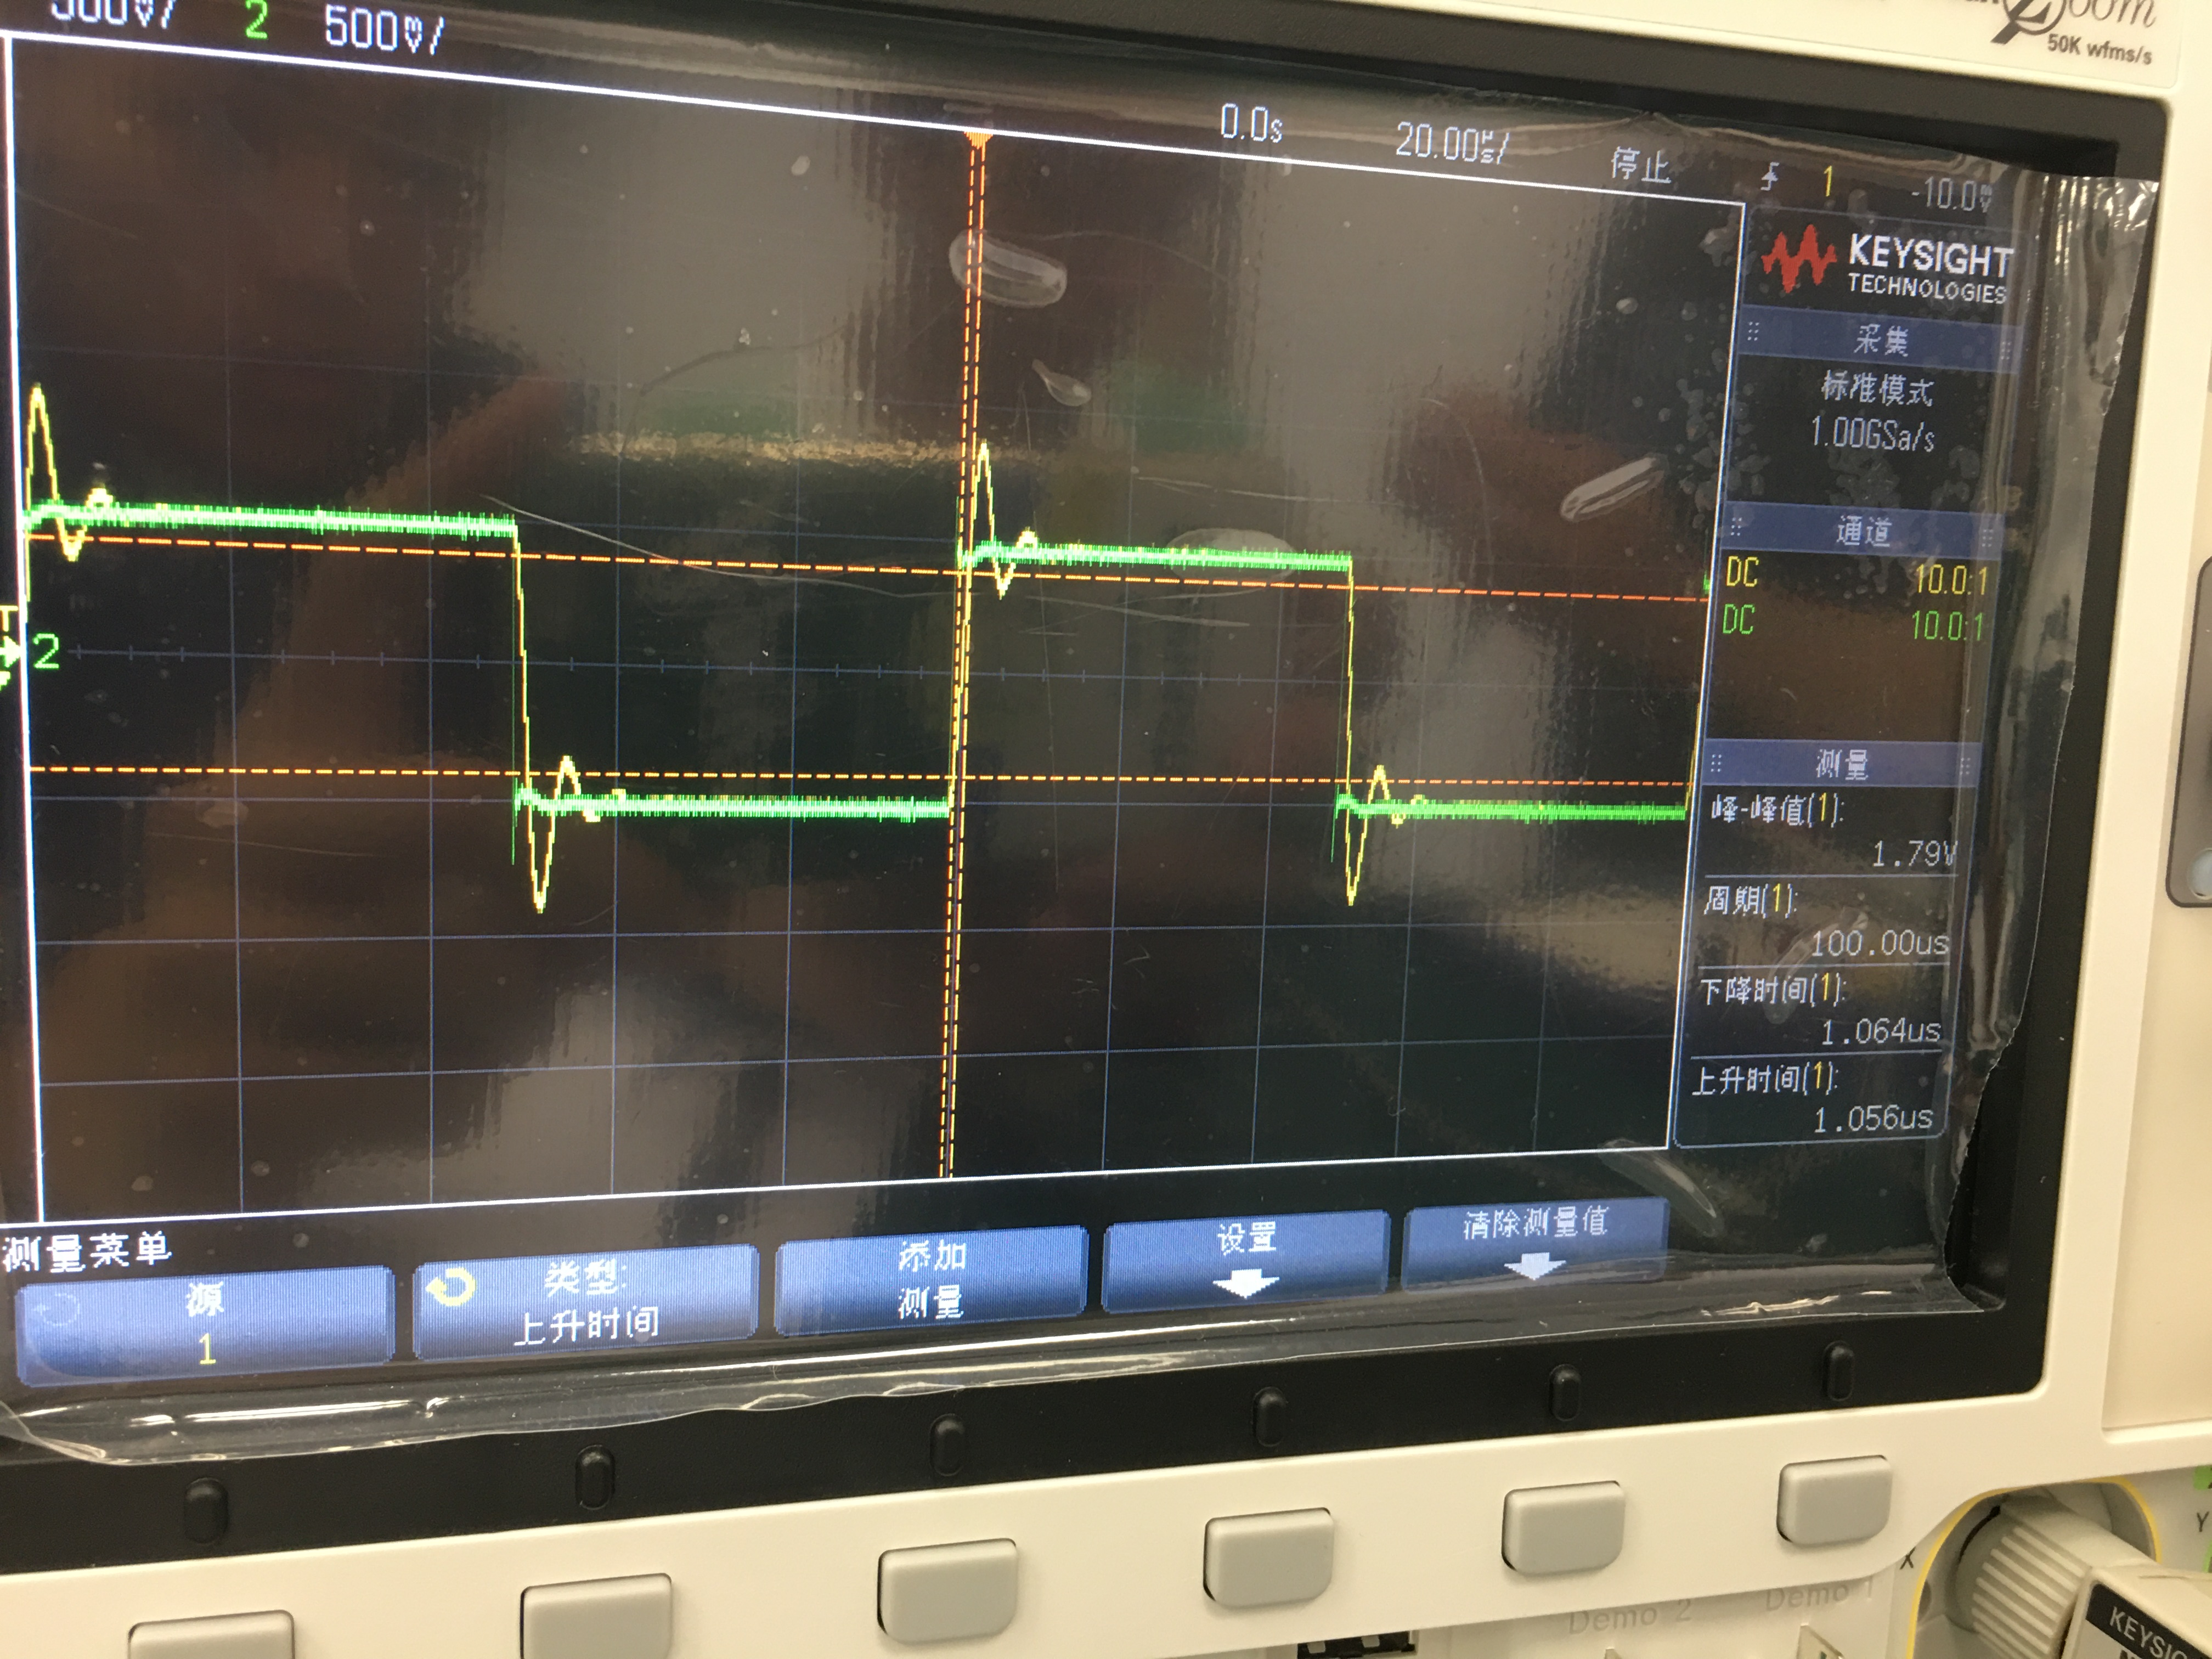
\includegraphics[width=.6\textwidth]{Figure3.jpg}
  \caption{Under-damped case}
  \label{img} 
\end{figure}
%--------------------------------- 

For the first under-damped circuit,
$$\omega=\frac{2\pi}{\Delta t}=2.094 \times10^6$$
According to the theoretical value, since at this time, the R we use is 0.481$k\Omega $ so that
$$\omega=\sqrt{\omega_0^2-\alpha^2}=\sqrt{\frac{1}{LC}-\frac{R^2}{4L^2}}=1.078\times10^6$$

The relative error is $94\%$. The reason of this great error will be discussed in the discussion part.

$$\delta_1=\frac{R}{2}\sqrt{\frac{C}{L}}=0.2181$$\\

For the second under-damped circuit,

$$\omega=\frac{2\pi}{\Delta t}=2.416\times10^6$$

Theoretically,

$$\omega=\sqrt{\omega_0^2-\alpha^2}=\sqrt{\frac{1}{LC}-\frac{R^2}{4L^2}}=1.102\times10^6$$

The relative error is $119\%$\\. Again, we observe that the relative error this time is still close to 1.

$$\delta_2=\frac{R}{2}\sqrt{\frac{C}{L}}=0.061$$\\

Since $\delta_1>\delta_2$, the damping in the first circuit decays faster.\\

For the critically damped circuit, the following figure shows the critically damped case.
 
%---------------------------------
  \begin{figure}[H]
  \centering
  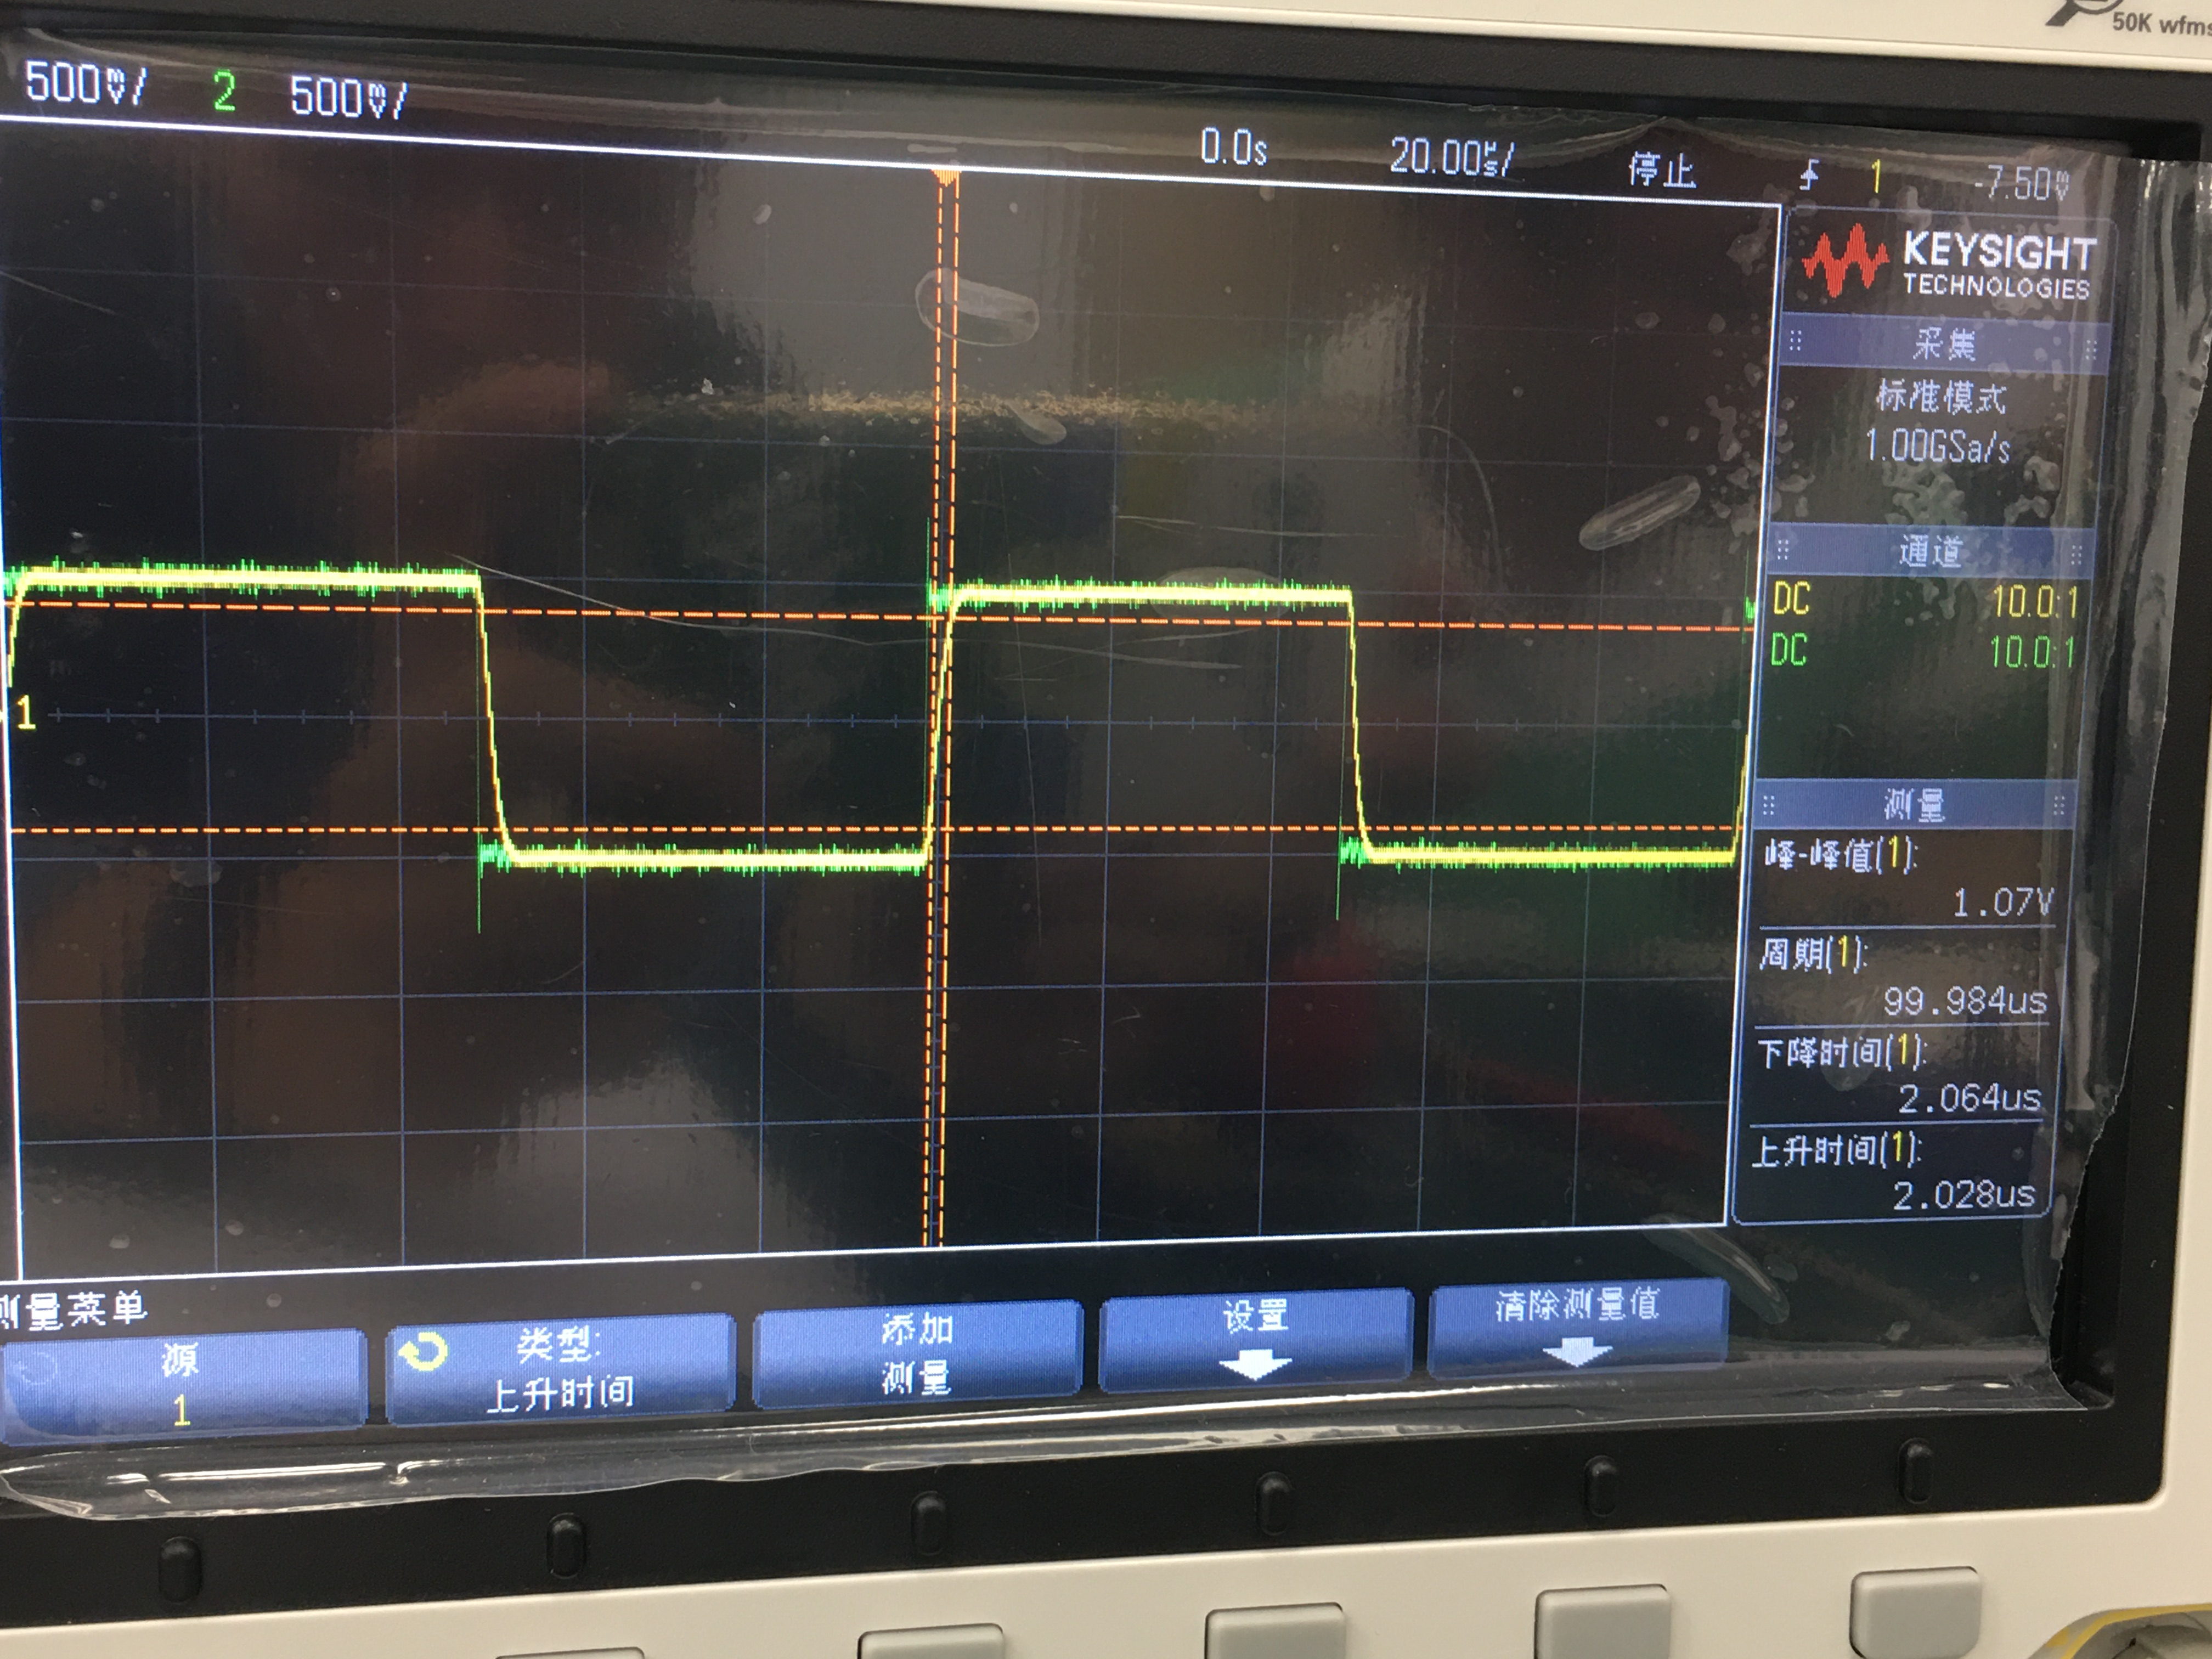
\includegraphics[width=.6\textwidth]{Figure4.jpg}
  \caption{Critically damped case}
  \label{img} 
\end{figure}
%--------------------------------- 
For the critically damped circuit,

$$R_{critical}=2\sqrt{\frac{L}{C}}=2208\Omega$$

\section{Conclusion}


In this experiment, we learned how to build a RC circuit and a RLC circuit and understood their properties such as the relationship between R,L,C and the time constant $\tau$. We also detect the $\delta$ in different kinds of circuit to compare the speed of decaying. 

However, in in the first part of the experiment which is the first order circuit, our relative error is very big. The error of both fastest circuit response and slowest circuit reponse are close to $65\%$. And we find that we may have used the wrong capacitor, we use the $820pF$ capacitor instead of the $0.1\mu F$.
\section{Reference}

Lab3\_Transient Lab\_Manual


\end{document}